\documentclass[12pt]{article}
\usepackage{enumerate}
\usepackage{notes}

\begin{document}
\title{Part A Linear Algebra}
\maketitle

\section*{Sheet 1}
\subsection*{} % 1
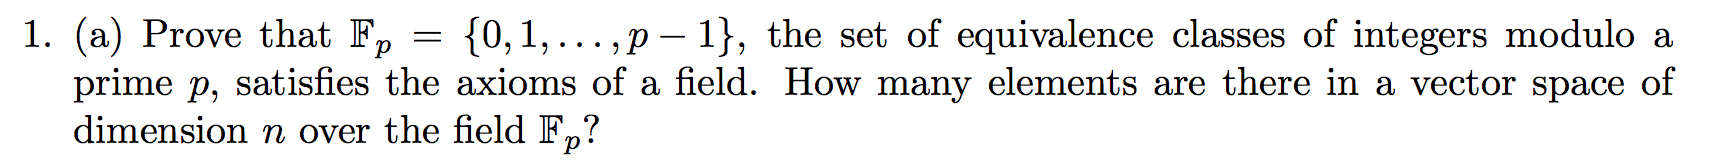
\includegraphics[width=450pt]{img/linear-algebra-a0-1-1-a.png}\\
\begin{mdframed}
  Let $a, b, c \in \Z$ with $0 \leq a < p, ~~ 0 \leq b < p, ~~ 0 \leq c < p$.

  Let $\bar a, \bar b, \bar c \in \F$ be equivalence classes of integers modulo $p$.

  The field axioms are listed below, together with proof that they hold for $\F_p$.
  \begin{enumerate}
  \item \textbf{Additive axioms}\\
    Define $\bar a + \bar b := \bar{a + b}$, then:
    \begin{enumerate}
    \item \textit{Existence of identity}: $\bar 0$ is the identity since
      $\bar a + \bar 0 = \bar{a + 0} = \bar{a}$ for all $\bar a \in \F_p$.
    \item \textit{Existence of inverses}: $(\bar a)^\1 = \bar{-a}$ since
      $\bar a + \bar{-a} = \bar{a + -a} = \bar{0}$ for all $a \in \F_p$.
    \item \textit{Commutativity}:
      $\bar a + \bar b = \bar{a + b} = \bar{b} + \bar{a}$ for all $a, b \in \F_p$.
    \item \textit{Associativity}:
      $\bar a + (\bar b + \bar c) = \bar a + \bar {b + c} = \bar{a + b + c} =
      \bar{a + b} + \bar{c} = (\bar a + \bar b) + \bar{c}$.
    \end{enumerate}
  \item \textbf{Multiplicative axioms}\\
    Define $\bar a ~ \bar b := \bar{ab}$, then:
    \begin{enumerate}
    \item \textit{Existence of identity}: $\bar 1$ is the identity since
      $\bar a \bar 1 = \bar{a\cdot 1} = \bar{a}$ for all $\bar a \in \F_p$.
    \item \textit{Existence of inverses for everything except additive
        identity}: We need to show that for all
      $\bar a \in \F_p \setminus \{\bar 0\}$ there exists $\bar b \in \F_p$
      such that $\bar a ~ \bar b = \bar 1$. \red{TODO: I couldn't think how to
        show this. I eventually allowed myself to google a little which brought
        up people pointing to the fact that since $a$ and $p$ are coprime,
        there exist $n, m$ such that $an + pm = 1$. Haven't thought about what
        to do with that yet.}
    \item \textit{Commutativity}:
      $\bar a ~ \bar b = \bar{ab} = \bar{b} ~ \bar{a}$ for all $a, b \in \F_p$.
    \item \textit{Associativity}:
      $\bar a (\bar b \bar c) = \bar a + \bar {bc} = \bar{abc} =
      \bar{ab}~\bar{c} = (\bar a ~ \bar b) \bar{c}$.
    \end{enumerate}
  \item \textbf{Distributive axiom}
    \begin{enumerate}
    \item \textit{Multiplication distributes over addition}: $\bar a (\bar b + \bar c) = \bar a (\bar{b + c}) = \bar{a(b+c)} = \bar{ab +
      ac} = \bar{ab} + \bar{ac} = \bar{a}~\bar{b} + \bar{a}~\bar{c}$
    \end{enumerate}
  \end{enumerate}

There are $p^n$ elements in a vector space of dimension $n$ over the field $\F_p$.
\end{mdframed}
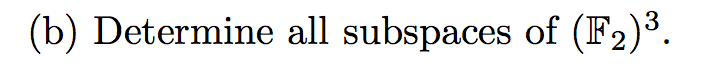
\includegraphics[width=250pt]{img/linear-algebra-a0-1-1-b.png}
\begin{mdframed}
  Note that
  \begin{align*}
    (\F_2)^3 = \{&\bar 0, \bar 1\}^3\\
             = \{&(\bar 0, \bar 0, \bar 0),\\
                 &(\bar 0, \bar 0, \bar 1),\\
                 &(\bar 0, \bar 1, \bar 0),\\
                 &(\bar 0, \bar 1, \bar 1),\\
                 &(\bar 1, \bar 0, \bar 0),\\
                 &(\bar 1, \bar 0, \bar 1),\\
                 &(\bar 1, \bar 1, \bar 0),\\
                 &(\bar 1, \bar 1, \bar 1)\}.
  \end{align*}
  The set of subspaces of $(\F_2)^3$ is
  \begin{align*}
    &\{\{(\bar 0, \bar 0, \bar 0)\}\} ~~~~~~~~~~~~~~~~~~~~~ \cup\\
    &\{\{(\bar 0, \bar 0, \bar 0), x\} ~|~ x \in (\F_2)^3\} ~~~ \cup\\
    &\{\{(\bar 0, a, b) ~|~ a, b \in \F_2\}\}  ~~~~~~~ \cup\\
    &\{\{(a, \bar 0, b) ~|~ a, b \in \F_2\}\}  ~~~~~~~ \cup\\
    &\{\{(a, b, \bar 0) ~|~ a, b \in \F_2\}\}  ~~~~~~~ \cup\\
    &\{(\F_2)^3\}.
  \end{align*}
\end{mdframed}


\end{document}
